% !TEX program = pdflatex
% TIST author instructions require acmsmall; author identity is pending.
\documentclass[acmsmall,review,anonymous]{acmart}
\acmJournal{TIST}
\setcopyright{none}
\settopmatter{printacmref=true}
\usepackage{kotex}
% pdfLaTeX: kotex uses its default Hangul fonts (UnBatang/UnDotum); no XeTeX font commands.
\usepackage{longtable,tabularx,algorithm,algpseudocode}
\usepackage{placeins}
\usepackage{xurl}
\usepackage{xcolor}
% Rule and condition names (small capitals), used consistently in text, tables and captions.
\newcommand{\agree}{\textsc{Agree}}
\newcommand{\allow}{\textsc{Allow}}
\newcommand{\literal}{\textsc{Literal}}
\newcommand{\witness}{\textsc{Witness}}
\newcommand{\witnessr}{\textsc{Witness-r}}
\newcommand{\review}{\textsc{Review}}
\newcommand{\direct}{\textsc{Direct}}
\newcommand{\refine}{\textsc{Refine}}
\newcommand{\rulesub}[1]{\text{\textsc{#1}}}
% Items the authors must complete before submission; printed in red so they cannot be missed.
\newcommand{\authortodo}[1]{\textcolor{red}{[#1]}}
\setlength{\emergencystretch}{2em}
% Review draft only: publisher assigns volume/issue/DOI/date after acceptance.
\title[Diagnosing Memory-Write Decisions]{Diagnosing Memory-Write Decisions in Conversational Assistants Through Specification-Based Replay}

% AUTHOR METADATA: pending, do not invent. Anonymous is a draft choice,
% not a claim that TIST mandates anonymous submissions. Once supplied,
% remove the anonymous option and add each author/affiliation/email/ORCID.
% Production DOI, copyright and volume/issue metadata come from ACM.
\begin{document}
\begin{abstract}
Conversational assistants with persistent memory must complete requested corrections without corrupting stored facts. A final-state score cannot show whether a difference between memory-write rules comes from the rule, an earlier stage, the reference's matching of written forms, or a lack of cases on which the rules could differ. Specification-based replay holds generated extractions and proposals fixed, varies only the admission rule, scores whole executed states, and counts exposure, the outputs on which rules can differ; exposure bounds any difference between two rules and confines the reference's influence on it to those outputs. On 48 Korean test cases and 21 model configurations, replay separates three confounds. A correction gain credited to evidence checks was the release of holds created by extraction, which a revised extraction instruction removed; most ties reflected zero exposure; and whether a gate on general-review proposals appears protective depends on the reference: accepting surface variants of required facts cuts the violations it avoids by almost two thirds and more than doubles its cost in completed changes, while comparisons among rules on fixed proposals are unchanged. Replay also explains a prespecified null result and, on real speech-recognition hypotheses, traces holds to genuine disagreement. An audit of ten memory-write evaluations shows that seven assess writes only through downstream answers.
\end{abstract}
\ccsdesc[500]{Computing methodologies~Discourse, dialogue and pragmatics}
\ccsdesc[300]{Computing methodologies~Nonmonotonic, default reasoning and belief revision}
\ccsdesc[300]{Computing methodologies~Intelligent agents}
\ccsdesc[100]{General and reference~Evaluation}
\keywords{conversational agents, persistent memory, memory correction, admission control, specification-based evaluation, failure diagnosis}
\maketitle

\section{Introduction}
Conversational assistants built on large language models increasingly keep a persistent memory of their users \cite{cite10}. Updating this memory requires both completing requested corrections and preserving facts that should remain unchanged. Current systems decide whether to add, revise, or delete stored facts \cite{cite4,cite6,cite21,cite39,cite40} and are usually evaluated later through questions about long conversations \cite{cite20,cite37}. Such a downstream or final-state score summarizes an outcome, but it does not identify which proposed write, admission decision, or reference convention produced it. This article studies that diagnostic gap.

A simple example illustrates the problem. Suppose that the stored opening year of a shop is 1991 and the reference requires a correction to 1993. The model proposes the correction, yet the application keeps 1991 because an agreement check does not find the corrected tuple in the facts extracted from every reading of the utterance. A rule that releases the hold completes the correction, but whether the credit belongs to that rule or to the extractor that omitted the tuple cannot be read from the final state.

We therefore separate generation, which produces a proposal; admission, which decides which proposed operations may execute; and execution, which changes the persistent state. Holding generation fixed and varying only admission makes every difference in the resulting state attributable to admission within the tested pipeline. Four rules then act on identical operations. \agree{} admits a correction only when its tuple is shared by the extracted facts of all readings, and \allow{} admits every correction that \agree{} holds for lack of shared support. Two evidence checks admit such a held correction only when its new value (\literal{}) or an affirmed quotation linked to the same target record (\witness{}) occurs in every reading. Because the rules can differ only on outputs that contain a held correction, we count these outputs and call the count \emph{exposure}.

Replay separates three confounds, each a pair of situations that a final-state score cannot distinguish (Figure~\ref{fig:1}). In the \emph{attribution} confound, a difference credited to the admission rule arises in another stage. In the \emph{specification} confound, an avoided reference violation reflects how the reference matches written forms rather than a semantic error. In the \emph{opportunity} confound, a tie reflects that no proposal reached the rules' decision boundary. Each has a precedent in state tracking: oracle analysis attributes errors to stages \cite{cite14}, and benchmark revisions list the surface variants of a value as equally correct \cite{cite44}. What is missing is a way to separate them for memory writes, which are judged on the whole executed state. Of ten memory-write evaluations that we audited, seven assess writes only through downstream answers, and none reports how many cases could distinguish the compared policies (Table~\ref{tab:1}).

Three research questions organize the study. RQ1 asks where admission can intervene and what produces the holds that it releases (Sections~6.1 and 6.2). RQ2 asks how evidence requirements change completion and reference violations on fixed proposals and how much these comparisons depend on the reference (Sections~6.3 and 6.4). RQ3 asks why a prespecified complete-pipeline test found no completion advantage and what changes with a learned verifier and with real recognition hypotheses (Sections~6.5--6.7).

\begin{figure}[tbp]
\centering
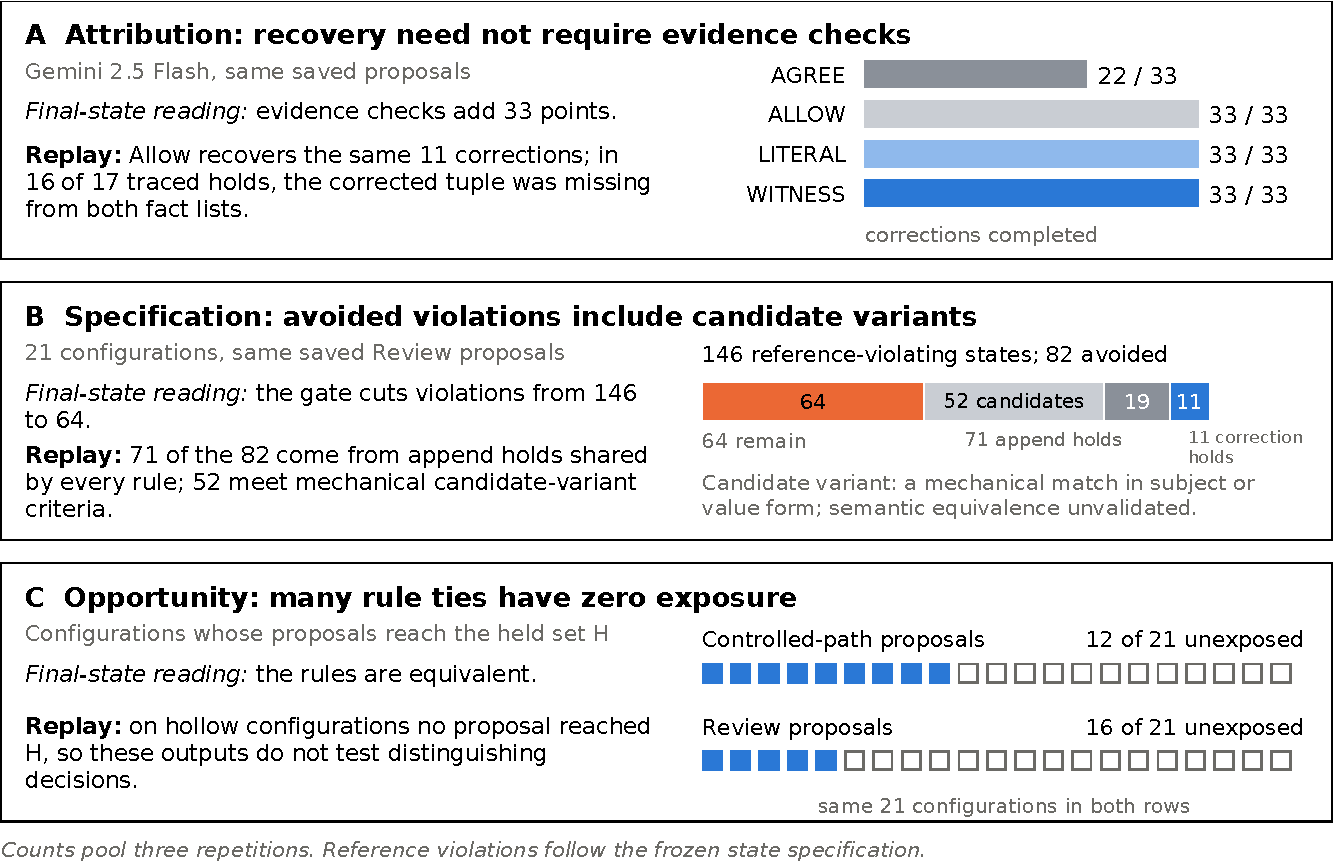
\includegraphics[width=\linewidth,height=.52\textheight,keepaspectratio]{media/figure_01.pdf}
\caption{Three evaluation confounds that a final-state score cannot distinguish: attribution (A), specification (B), and opportunity (C). Each row sets what the final-state score shows beside what replay of the same saved artifacts shows. A: Gemini 2.5 Flash, strict corrections completed out of 33 observations under each rule. B: The 146 reference-violating states under \review{} on the 21-configuration panel, split by whether the gate avoids them and, if so, by the held operation; ``variants'' are append holds whose tuple differs from a required fact only in subject label, spacing, or value form (Section~6.4). C: The 21 panel configurations, with controlled-path and with \review{} proposals; hollow squares mark configurations on which no proposal reached the held set $H$.}\label{fig:1}
\Description{Three evaluation confounds that a final-state score cannot distinguish. A, attribution: On Gemini 2.5 Flash, Agree completes 22 of 33 corrections and Allow, Literal, and Witness each complete 33; in 16 of 17 traced holds the corrected tuple was missing from both fact lists. B, specification: Of 146 reference-violating states under Review, the gate avoids 82, of which 71 come from append holds shared by every rule and 11 from correction holds; 52 of the 71 hold a variant of a required fact; 64 remain. C, opportunity: On 12 of 21 configurations with controlled-path proposals and on 16 of 21 configurations with Review proposals, no proposal reached the held set, so the rules were never compared on a decision.}
\end{figure}

This article makes three contributions:
\begin{itemize}
\item \emph{Specification-based replay with exposure.} The protocol extends fixed-candidate replay \cite{cite51} to edits of identified records under competing readings, scores whole executed states, and counts exposure. Exposure bounds any difference between two rules on the same proposals and confines the reference's influence on that difference to the exposed outputs (Proposition~\ref{prop:1}). The protocol runs on saved artifacts: across 21 configurations and 3,024 episodes, a re-executed gate reproduces every saved score, and the same machinery replays a learned verifier and recognizer hypotheses (Sections~4--6).
\item \emph{Three confounds, each traced to a cause and tested.} Extraction, not the evidence check, produced the held corrections that the checks were credited with releasing, and a revised extraction instruction removed them; zero exposure explained most ties; and the reference decided whether a gate looked protective (Sections~6.1--6.4). On real recognition hypotheses, the same trace returned a different cause, disagreement between hypotheses (Section~6.7).
\item \emph{A robustness analysis of the reference.} Re-scoring every episode under a reference that accepts surface variants of required facts separates the conclusions that hold under both references, namely all comparisons among rules on fixed proposals, from those that do not: the apparent safety of a gate on general-review proposals and the direction of the complete-pipeline comparison (Sections~6.4 and 6.5).
\end{itemize}
\emph{Scope of claims.} The claims are existence and attribution claims, established by traced artifacts whose counts are exact and reproducible; how often each confound arises in other systems is a separate question (Section~8).

\section{Related Work}
\subsection{Memory Updates and Admission in LLM Agents}
Several systems give LLM agents a persistent memory that is updated through explicit operations. MemGPT treats the context window as fast memory and moves information to and from external storage through function calls \cite{cite21}. Mem0 extracts candidate facts and applies one of four operations to existing memories: add, update, delete, or no operation \cite{cite6}. A-Mem stores memories as linked notes whose attributes are revised as new notes arrive \cite{cite39}, and MemoryBank, recursive summarization, SeCom, LD-Agent, and Generative Agents maintain or select conversational history in related ways \cite{cite15,cite22,cite23,cite35,cite47}. Closest to the correction decision studied here, Bae et al.\ cast memory management in Korean long-term conversation as pairwise operations between a stored sentence and a new session summary (pass, replace, append, or delete) \cite{cite4}. They compared trained classifiers with natural language inference models mapped to these operations and evaluated operation accuracy, set-level overlap, and human ratings of later sessions. Memory-R1 learns add, update, delete, and no-operation decisions from a reward based on downstream answer correctness \cite{cite40}, and Zep invalidates, rather than deletes, knowledge-graph edges that newer information contradicts \cite{cite26}.

A recent line of work treats the write itself as an admission decision. A-MAC learns an admission policy from interpretable factors (future utility, factual confidence, semantic novelty, temporal recency, and a content-type prior) and evaluates admission decisions against labeled candidate memories \cite{cite48}; ConsistencyGate samples the same model several times to score whether a candidate fact is supported by its source and admits the fact above a threshold \cite{cite49}; and DerivAudit audits whether a stored memory follows from the history available when it was written, finding that support often lies beyond the writer's citations and that verifiers still admit many unsupported memories \cite{cite51}. STALE evaluates whether agents notice that a stored memory has been implicitly invalidated by later information \cite{cite50}. Memory writes are also an attack surface: AgentPoison and MINJA show that poisoned or injected records, the latter inserted through ordinary queries, later steer agent behavior \cite{cite5,cite7}. In our setting, the surrounding history is supplied rather than retrieved, so retrieval failure is not confounded with admission failure; how the position of information affects its use is a separate question \cite{cite16}.

\subsection{State Revision and Competing Hypotheses}
Dialogue-state tracking already models state revision. SOM-DST predicts an operation for each slot before generating values \cite{cite14}, and its oracle analysis attributes most errors to the operation predictor rather than to value generation, an early stage-level diagnosis of the kind we apply to memory writes. AG-DST amends an initially generated state \cite{cite33}, dataflow synthesis supports executable dialogue programs and non-destructive revision \cite{cite3}, and PoA generates semantic-action code that updates the dialogue state \cite{cite31}. Other trackers select the relevant turns, suppress incorrect values, or rewrite queries to resolve coreference \cite{cite11,cite17,cite34}. The second Dialog State Tracking Challenge supplied competing speech-recognition hypotheses for every turn and scored the tracked state turn by turn \cite{cite12}; its setting is close to ours, although there the tracker produces the state itself, and Section~6.7 replays our admission rules on its hypotheses. MultiWOZ~2.2 removes values that the system offered before the user accepted them \cite{cite44}, and MultiWOZ~2.4 removes values that only the system mentioned \cite{cite42}; both revisions show why the timing and source of evidence matter. MultiWOZ~2.2 also lists the surface variants of a value as equally correct \cite{cite44}, a reminder that an exact-match reference can count an equivalent mention as an error (Section~6.4 returns to this issue). Our comparison intervenes after extraction and proposal are fixed: it evaluates the permission to execute a proposal and thus complements these state-generation methods.

\subsection{Evidence, Clarification, and Evaluation}
Clarification has long been modeled as a decision under uncertainty \cite{cite43,cite24,cite8,cite9,cite45}, although human clarification is only weakly tied to annotated ambiguity \cite{cite19} and is not mirrored by model uncertainty \cite{cite32}; an uncertain detail can be unnecessary for the next action yet consequential for a durable write. Disagreeing readings resemble the inter-context conflicts studied between retrieved sources \cite{cite38}, and a quoted span shows that a value occurs in the source, not that it supports the proposed fact \cite{cite1}; this distinction motivates comparing literal evidence with target-linked witnesses. Attribution to identified sources can be defined and rated by people \cite{cite25}, entailment-based checkers detect factual inconsistency \cite{cite13}, LLM judges can approximate human preferences \cite{cite46}, and agreement across readings resembles self-consistency over sampled outputs \cite{cite36}. $\tau$-bench scores agents by the final database state after tool use \cite{cite41}, the kind of executed-state endpoint that we apply to a single turn. Self-Refine and Reflexion revise outputs at inference time \cite{cite18,cite29}; we use a two-call general review as the alternative complete pipeline, and because the choice of instruction can itself change results \cite{cite2}, every condition receives the same task facts and retention constraints. Automatic and human assessments can agree \cite{cite30} or rank systems differently \cite{cite28}, so agreement has to be established for each endpoint. Table~\ref{tab:1} audits what memory-write evaluations report.

\begin{table}[tbp]
\centering
\caption{Reporting audit of ten memory-write evaluations, from what each paper reports. \emph{Fixed}: the compared write or admission policies act on the same generated candidates. \emph{Both errors}: missed required writes and wrongly admitted writes are reported, not only downstream answers. \emph{Opportunity}: the number of cases on which the compared policies could, or did, differ. \emph{Matching}: how outputs are compared with references; n.r., not reported.}\label{tab:1}
\footnotesize
\setlength{\tabcolsep}{3pt}
\begin{tabular}{@{}>{\raggedright\arraybackslash}p{\dimexpr0.19\linewidth-5pt\relax}>{\raggedright\arraybackslash}p{\dimexpr0.22\linewidth-5pt\relax}>{\raggedright\arraybackslash}p{\dimexpr0.09\linewidth-5pt\relax}>{\raggedright\arraybackslash}p{\dimexpr0.10\linewidth-5pt\relax}>{\raggedright\arraybackslash}p{\dimexpr0.135\linewidth-5pt\relax}>{\raggedright\arraybackslash}p{\dimexpr0.265\linewidth-5pt\relax}@{}}
\toprule
\textbf{Work} & \textbf{Write decision scored} & \textbf{Fixed} & \textbf{Both errors} & \textbf{Opportunity} & \textbf{Matching} \\
\midrule
MemoryBank \cite{cite47} & Downstream answers & -- & -- & -- & Human ratings; agreement n.r. \\
MemGPT \cite{cite21} & Downstream answers & -- & -- & -- & LLM judge and ROUGE-L; agreement n.r. \\
Mem0 \cite{cite6} & Downstream answers & -- & -- & -- & Token overlap and LLM judge; agreement n.r. \\
A-Mem \cite{cite39} & Downstream answers & -- & -- & -- & Token and embedding overlap \\
Zep \cite{cite26} & Downstream answers & -- & -- & -- & LLM judge \\
Memory-R1 \cite{cite40} & Downstream answers & -- & -- & -- & Token overlap and LLM judge \\
STALE \cite{cite50} & Downstream probes & -- & Partial & -- & LLM judge with human check \\
Bae et al. \cite{cite4} & Operation per memory pair & Yes & Partial & -- & Human labels, majority of three \\
A-MAC \cite{cite48} & Admission per candidate & Yes & Yes & -- & Candidate labels; process n.r. \\
ConsistencyGate \cite{cite49} & Admission per fact & Partial & Yes & -- & Constructed labels \\
\addlinespace[2pt]
This work & Admission, whole state & Yes & Yes & Yes & Exact and variant-tolerant reference; no human agreement \\
\bottomrule
\end{tabular}
\end{table}

DerivAudit compares verification settings on the same candidate memories and reports both supported-memory retention and unsupported admission \cite{cite51}, so replaying fixed candidates is not in itself our contribution. We add edits of identified records under competing readings, whole-state scoring, exposure with its bound, and an analysis of how far each conclusion depends on the reference. We do not compare directly with A-MAC or ConsistencyGate, which score the admission of candidate facts against labels rather than whole executed states; Section~6.6 instead adds a learned verifier as a further rule on the same proposals.

\section{Task and Decision Boundary}
A test case is $x=(h,T,M,\pi)$, consisting of the preceding context $h$; an indexed sequence $T=(t_1,\ldots,t_k)$ of alternative readings of one current utterance, which may coincide; an initial memory state $M$; and a case-level retention permission $\pi$. The readings are simultaneous alternatives for the same speaker's turn, not separate speakers or successive turns. A record has a persistent identifier and a fact tuple (subject, relation, value, time). The model proposes an action $a$, a reply $u$, and an ordered list of memory operations $Q$; the application executes the admitted operations in one transaction and returns the state $M'$ together with an execution log $\rho$.

Four operations are available: APPEND, CORRECT, HOLD, and no-write. A correction targets an existing record and replaces its value while keeping its identifier, whereas a hold leaves a proposed fact uncommitted. Retention permission is separate from factual support, because a clearly stated fact may still be disallowed for storage. Supplying the initial state lets the evaluation distinguish a new fact from an obsolete or protected one without having to infer it. For each case, the reference specifies the allowed actions, the required and forbidden tuples, the records that must remain unchanged, the obsolete versions to retire, and any records that must no longer appear; all of these requirements are checked on the executed state.

We assess required change and preservation together. On a positive case, at least one required fact is absent or an obsolete version must be retired, so holding every proposal fails. A correct target update can still fail whole-state conformity when it also appends a fact outside the requested edit. We score the action and persistent state against the reference and inspect reply--state discrepancies in selected traces; reply truthfulness is not a scored endpoint. In tables, ``Viol.'' abbreviates reference violations. Table~\ref{tab:2} defines the terms and endpoints used throughout.

\begin{table}[tbp]
\centering
\caption{Terms and endpoints. With three repetitions, the correction, positive, and all-case denominators are 33, 84, and 144 per configuration; with one repetition, they are 11, 28, and 48.}\label{tab:2}
\small
\setlength{\tabcolsep}{3pt}
\begin{tabular}{@{}>{\raggedright\arraybackslash}p{\dimexpr0.2727\linewidth-1.64pt\relax}>{\raggedright\arraybackslash}p{\dimexpr0.7273\linewidth-4.36pt\relax}@{}}
\toprule
\textbf{Term} & \textbf{Definition} \\
\midrule
Reading & One written alternative of the current utterance, supplied as text. \\
Extraction $F$ & Reading-level fact lists and correction witnesses produced by the first model call. \\
Proposal $(a,u,Q)$ & Action, reply, and memory operations produced by the second model call. \\
Held set $H$ & CORRECT operations that \agree{} holds only for lack of shared support, although the extraction validly covers every reading. \\
Exposure & Outputs on which the rules can decide differently, that is, outputs that contain an operation in $H$, reported with the number of distinct cases they represent. \\
Complete pipeline & A system that generates its own proposal. \review{}: a draft plus one general-review call. \\
Controlled path & Extraction, proposal, and \witness{} admission; reply rendered from the execution log. \\
Strict correction completion & Allowed action and exactly the reference-specified whole state on the 11 correction cases. \\
Positive-change completion & Allowed action and exact whole state on the 28 positive cases (the prespecified primary endpoint). \\
Reference-violating state & Forbidden or extra write, or damage to a protected fact, as defined by the reference (all 48 cases). \\
Whole-state conformity & Executed state meeting every state requirement of the reference (all 48 cases). \\
Negative preservation & Preservation of the state on the 20 cases that require no change. \\
\bottomrule
\end{tabular}
\end{table}

\section{Correction Admission Rules}
\subsection{One Proposal and Four Admission Decisions}
The controlled path makes two model calls. The first returns an extraction $F$: for each reading, the atomic facts that the reading supports, and, for each pair of a stored record and a reading, one correction witness with a polarity label (affirmed, negated, uncertain, or absent), a new value, and a verbatim quotation. The second call receives the test case together with $F$, marked as fallible, and generates the final proposal. Every admission rule receives the identical test case, extraction, and proposal, together with an isolated copy of $M$, so changing the rule requires no further model call (Figure~\ref{fig:2}).

\begin{table}[tbp]
\centering
\caption{Admission rules applied to the same proposal. Outside $H$, every rule keeps \agree{}'s decision; retention permission and execution checks are shared.}\label{tab:3}
\small
\setlength{\tabcolsep}{3pt}
\begin{tabular}{@{}>{\raggedright\arraybackslash}p{\dimexpr0.1667\linewidth-1.00pt\relax}>{\raggedright\arraybackslash}p{\dimexpr0.8333\linewidth-5.00pt\relax}@{}}
\toprule
\textbf{Rule} & \textbf{Admission within $H$} \\
\midrule
\agree{} & Keeps the conservative hold when shared extracted support is missing. \\
\allow{} & Admits every otherwise eligible correction in $H$. \\
\literal{} & Checks the existing target and the unchanged subject, relation, and time; requires the new value in every reading and current-turn evidence. \\
\witness{} & Additionally requires one affirmed, matching, target-linked witness per reading, supported by an exact source quotation that contains the value. \\
\bottomrule
\end{tabular}
\end{table}

\agree{} applies to every proposed APPEND and CORRECT operation. It admits an operation when the exact subject--relation--value--time tuple is supported by the fact list of every reading or is already present in $M$; otherwise, it changes the operation to HOLD. \agree{} was the conservative gate of the original protocol, fixed before collection, and is meant to keep a fact out of memory when the readings disagree about it. Shared support requires that the extraction validly cover all readings. Because the test compares tuples exactly as extracted, and because the extraction schema allows a reading's fact list to be empty, a correction can appear in the proposal and in the witnesses yet be missing from the intersection of the extracted fact lists. This is how the held set arises.

Let $H(x,F,Q)$ be the set of operation indices $j$ for which \agree{} holds a proposed CORRECT only because its support is not shared, although every reading is validly covered. All differences between \agree{} and the other three rules lie within $H$; outside $H$, every rule keeps \agree{}'s decision (Table~\ref{tab:3}). \allow{} restores every correction in $H$ and nothing else, so an APPEND that lacks shared support stays held under every rule. Two predicates define the evidence checks. For \literal{} ($L_j=1$), the proposal must name one existing target; preserve its subject, relation, and time; change its value; and cite the current turn in both the fact and the operation. In addition, the replacement value must occur literally in every reading. For \witness{} ($W_j=1$), the same target and source conditions must hold, and each reading must supply exactly one witness for the target record that is labeled affirmed, repeats the proposed subject, relation, time, and value, cites the current turn, and quotes a verbatim span of that reading containing the replacement value. The application verifies the structure and linkage of these model-generated witnesses, but the polarity label itself is taken from the model.

Two examples show how the checks differ. The sentence ``the shop opened in 1993, not 1991'' satisfies both checks for an opening-year record. By contrast, ``My son works at Daehan Post'' satisfies the literal check for an update of the speaker's own workplace but should fail the witness check, which requires every reading to affirm the value for the targeted record: the affirmed statement concerns the son.

\subsection{Containment and the Opportunity to Intervene}
The admitted sets of the four rules are nested. Write $A_X$ for the indices in $H$ that rule $X$ admits; then
\begin{equation}
A_{\rulesub{Witness}}=\{\,j\in H : W_j=1\,\}\;\subseteq\; A_{\rulesub{Literal}}=\{\,j\in H : L_j=1\,\}\;\subseteq\; A_{\rulesub{Allow}}=H .
\label{eq:containment}
\end{equation}
The first inclusion holds because a passing witness carries the required target and source linkage and an exact quotation that contains the value, so the value occurs in every reading; the second follows from the restriction to $H$. This ordering concerns admitted operations only. It need not carry over to final-state accuracy when a transaction is rejected, when operations interact, or when a witness is wrong.

\agree{} and \allow{} are therefore the two ends of this ordering rather than competing designs: no rule that acts on $H$ can admit more held corrections than \allow{} or fewer than \agree{}. We compare \literal{} and \witness{} with both ends: with \allow{} for the reference violations they prevent, and with \agree{} for the corrections they recover and the reference violations they add. Because \agree{} reads model-extracted facts, its holds can originate in extraction rather than in disagreement between readings; the saved extraction shows which of the two occurred (Section~6.1). \witness{} and \literal{} decide differently only on $K=\{\,j\in H : L_j=1,\ W_j=0\,\}$, where a hold may either protect the correct state or keep an obsolete fact unnecessarily. When $H$ is empty, all four rules must agree. The following bound makes this precise for any two rules and any endpoint.

\begin{proposition}[Exposure bound and reference dependence]\label{prop:1}
Let rules $X$ and $Y$ act on the same $N$ outputs, and let $E$ be the set of outputs that contain an operation on which $X$ and $Y$ can decide differently. For every endpoint indicator $S$ computed on the executed state, (i) $|\bar S_X-\bar S_Y|\le |E|/N$, and (ii) the difference $\bar S_X-\bar S_Y$ depends on the reference only through the scores of the outputs in $E$.
\end{proposition}
\begin{proof}
Outside $E$, the two rules admit the same operations, so the deterministic executor produces the same state and $S$ takes the same value under $X$ and $Y$. Hence $N(\bar S_X-\bar S_Y)=\sum_{o\in E}\bigl(S_X(o)-S_Y(o)\bigr)$, which is at most $|E|$ in absolute value and involves the reference only through outputs in $E$.
\end{proof}

For the four rules, $E$ is the set of outputs that reach $H$; for a gate applied to proposals that were not gated before, $E$ contains every output with a held APPEND or CORRECT or an invalid extraction. Exposure therefore sets the resolution of a comparison: with 11 exposed outputs among 144, no rule comparison can exceed 7.6 percentage points, and with none, a tie carries no information about the rules. Part~(ii) predicts which comparisons a change of reference can move, which Section~6.4 tests.

\begin{figure}[tbp]
\centering
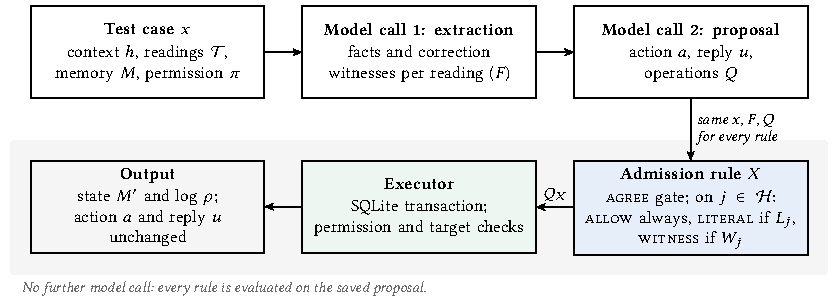
\includegraphics[width=\linewidth,height=.42\textheight,keepaspectratio]{media/figure_02.pdf}
\caption{Fixed-proposal architecture. Two generation calls produce one extraction and one proposal. Each admission rule is then applied to the same artifacts and executed on an isolated copy of the initial state.}\label{fig:2}
\Description{Fixed-proposal architecture. Two generation calls produce one extraction and one proposal. Each admission rule is then applied to the same artifacts and executed on an isolated copy of the initial state.}
\end{figure}

\subsection{Execution and Complete Pipelines}
The application applies operations transactionally to a separate SQLite state for each rule and records read-after-write execution logs; the executor enforces retention permission and target existence for every rule. Because admission does not regenerate the action or the reply, differences in state outcomes between rules can be assigned to admission alone within this pipeline. For the same reason, a held write can coexist with a reply that asserts the held value (Online Appendix~H), and the unchanged reply is not credited to admission. \witness{} uses the same two calls per output as \agree{}, and \allow{} and \literal{} are computed from the saved proposals (Algorithm~\ref{alg:1}; Online Appendix~C).

The comparison pipeline, \review{}, generates its own proposal from a draft and one general-review call, so it and the controlled path use the same number of calls. The original protocol also ran a single direct draft and one draft--feedback--refine cycle adapted from Self-Refine \cite{cite18}; they share \review{}'s initial draft where the design permits and are reported in Online Appendices~A and F. The prespecified primary test compares the controlled path, with its reply rendered from the execution log, with \review{}. Rendering does not change any state endpoint, so the tables report the common state score under \witness{} (Online Appendix~A).

\begin{algorithm}[tbp]
\caption{Admission on a fixed proposal. Reply rendering is a separate downstream option.}\label{alg:1}
\begin{algorithmic}[1]
\Require case $x=(h,T,M,\pi)$, extraction $F$, proposal $(a,u,Q)$, rule $X$ (\agree{}, \allow{}, \literal{}, or \witness{})
\Ensure action $a$ and reply $u$ unchanged; executed state $M'$ and log $\rho$
\If{$Q$ fails schema validation}
  \State \Return $(a,u,M,\emptyset)$ \Comment{no write; scored as an invalid output}
\EndIf
\State $Q_X \gets \textsc{AgreeGate}(x,F,Q)$ \Comment{holds APPEND and CORRECT without shared support}
\ForAll{$j\in H(x,F,Q)$}
  \If{$X=\allow$ \textbf{or} ($X=\literal$ \textbf{and} $L_j=1$) \textbf{or} ($X=\witness$ \textbf{and} $W_j=1$)}
    \State $Q_{X,j}\gets Q_j$ \Comment{restore the proposed correction}
  \EndIf
\EndFor
\State $(M',\rho)\gets \textsc{Execute}(M,Q_X,\pi)$
\State \Return $(a,u,M',\rho)$
\end{algorithmic}
\end{algorithm}

\section{Evaluation Design}
\subsection{Sources and Model Configurations}
The main source contains 60 Korean test cases written by the authors with AI assistance: 12 development cases and 48 held-out cases spanning 12 problem families of four cases each (Online Appendix~A, Table~A3). Each held-out case was run three times per model configuration. A private reference, fixed before the main collection, specifies the requirements listed in Section~3, including the distinction between replacing a value and removing its record. The collection script received the public cases but not the reference, and the configurations, prompts, admission rules, and evaluator were fixed in a frozen protocol before collection. We use Korean because widely used memory benchmarks are in English \cite{cite20,cite37} and because Korean writing yields several surface forms of one fact (word spacing varies in practice, and a person may be named by a kinship term, a given name, or both), which stresses exact tuple matching (Section~6.4).

All alternative readings of the main source are written text authored with AI assistance. Within a case, they can be identical, differ in surface form, or differ in value, person, or polarity; they play the role of competing recognition hypotheses but were not produced by a recognizer, so how often they reach the held set characterizes this source rather than any recognizer.

The original protocol planned a Holm-adjusted primary comparison for five model families; Gemini 2.5 Flash, Llama 3.1 8B, and Qwen3 14B (local 4-bit) were collected, and two families were not (Online Appendix~C). Six later Gemini configurations reuse the 48 cases and were added after the earlier results had been inspected. The model panel comprises the 21 configurations that completed all 48 cases in all three repetitions with at least 95\% valid final outputs in both \review{} and the controlled path: seven Gemini, eight Claude, and three GPT configurations together with DeepSeek 3.2, GLM 5, and Qwen3 14B, for 3,024 case-repetition episodes. This validity criterion was set after collection and applies to complete pipelines, not semantic outcomes; of the 28 configurations with complete triplets, seven fall below it, among them Llama 3.1 8B (Online Appendix~G). Model labels denote recorded provider or runtime configurations and do not imply matched parameter counts, precision, or reasoning budgets.

Table~\ref{tab:4} lists the further sources. Three authored or adapted sources probe transfer and are reported in Online Appendices~D--F: a 24-case contrast set written after the initial finding by a separate agent that saw neither the rule code nor earlier outputs, a 12-case boundary probe, and 16 selected MultiWOZ~2.4 turns \cite{cite42}. A fourth source, 48 user turns from the DSTC2 test set, supplies real speech-recognition hypotheses with a reference derived from human-reviewed labels (Section~6.7). Three follow-up runs, collected after the results above had been inspected and fixed before their outputs, test the diagnoses (Online Appendix~J): a revised extraction instruction on the held cases, a learned verifier (Gemini 3.1 Pro Preview) that approves or holds each APPEND and CORRECT in saved \review{} proposals without seeing the extraction or the reference, and the DSTC2 replay.

\begin{table}[tbp]
\centering
\caption{Sources and their roles. Additional configurations reuse the main cases, and each source keeps its own denominators.}\label{tab:4}
\small
\setlength{\tabcolsep}{3pt}
\begin{tabular}{@{}>{\raggedright\arraybackslash}p{\dimexpr0.2727\linewidth-4.91pt\relax}>{\raggedright\arraybackslash}p{\dimexpr0.0909\linewidth-1.64pt\relax}>{\raggedright\arraybackslash}p{\dimexpr0.1364\linewidth-2.45pt\relax}>{\raggedright\arraybackslash}p{\dimexpr0.5000\linewidth-9.00pt\relax}@{}}
\toprule
\textbf{Source} & \textbf{Cases} & \textbf{Repetitions} & \textbf{Role} \\
\midrule
Main Korean cases & 48 & 3 & Fixed-proposal and complete-pipeline comparisons \\
DSTC2 test turns & 48 & 1 & Real recognition hypotheses; 41 callers \\
Contrast set & 24 & 1 & 12 supported and 12 unsupported edits \\
Boundary probe & 12 & 1 & Six paired edits; no exposure \\
Public dialogue probe & 16 & 1 & 10 eligible self-repairs; six unscored \\
Follow-up runs on main cases & 5; 48 & 1 & Revised extraction; learned verifier \\
\bottomrule
\end{tabular}
\end{table}

\subsection{Endpoints and the Variant-Tolerant Reference}
The primary endpoint prespecified in the original study is positive-change completion: joint success of the action and the whole state on the 28 of the 48 main cases that require a new fact or the retirement of an obsolete version. A successful output must be valid, choose an allowed action, contain the required facts, omit forbidden and obsolete tuples, preserve protected facts, satisfy the required removals, and introduce no unlisted fact; provider failures and invalid outputs stay in the denominator. Strict correction completion applies the same criterion to the 11 correction-eligible cases. The reference-violation endpoint flags forbidden or extra writes and damage to protected facts across all 48 cases. Successful positive changes and reference-violating states are always reported together, so that withholding more operations is not mistaken for improving the task.

The reference matches tuples exactly, so an unlisted fact counts as a violation even when it restates a required fact in another form. To measure how much each conclusion depends on this convention, we re-scored every saved output under a \emph{variant-tolerant reference}. A tuple counts as a required or protected fact when its relation and time match and, after Unicode NFC, case folding, and whitespace removal, its subjects are equal, both denote the participant, or one contains the other, and its values are equal or one contains the other; a participant label is never matched to another person's label. Forbidden and obsolete tuples stay exact, so the second reference can only credit outputs. It accepts 38 distinct pairs in 10 cases, all listed in Online Appendix~K, and the scorer reproduces every archived score of the exact reference. It is a mechanical convention, not a semantic judgment, and no human rated equivalence.

\subsection{Paired Analysis}
For configuration $m$ and case $i$, the paired difference is $d_{mi}=\tfrac{1}{3}\sum_{r=1}^{3}\bigl[Y_{mir}(\mathrm{ctrl})-Y_{mir}(\rulesub{Review})\bigr]$, where $Y$ is the endpoint indicator for repetition $r$ and ctrl denotes the controlled path; the effect estimate averages $d_{mi}$ over cases. Uncertainty is reported as 95\% percentile intervals from 5,000 case-cluster bootstrap draws that keep the repetitions, and for pooled estimates the configurations, of a case together (48 clusters for all-case endpoints, 28 for positive completion, and 11 for correction completion). The prespecified exact two-sided McNemar test counts a case as a success when it succeeds in at least two of three repetitions, and the original plan adjusted the five planned family tests with Holm's method (Online Appendix~A). Each original-protocol run made $48\times3\times6=864$ physical calls, of which each two-call pipeline used 288, without retries. Gemini 2.5 Flash used temperature 0.2, disabled thinking, and 2,048 output tokens; later configurations used their supported thinking settings, so the panel compares configurations as run rather than at equal compute (Online Appendix~C). Counts pool configurations and repetitions, which are not independent replications of a case; distinct cases are reported alongside.

\subsection{Confirmatory and Exploratory Analyses}
Only the comparison of the controlled path with \review{} was prespecified as a test; the study began as that test, and the replay analyses were added to explain its outcome (Table~\ref{tab:5}). Applying the gate to saved general-review proposals pairs each saved \review{} proposal with the extraction from the same configuration, case, and repetition, applies one of the four rules, and executes the result with the frozen executor; we write \review{}+\witness{} and so on. These conditions, two string-normalization controls, the variant audit, and the variant-tolerant re-scoring required no model call (Online Appendices~I and K).

\begin{table}[tbp]
\centering
\caption{Status of the reported analyses. ``Prespecified'' does not imply public preregistration.}\label{tab:5}
\small
\setlength{\tabcolsep}{3pt}
\begin{tabular}{@{}>{\raggedright\arraybackslash}p{\dimexpr0.5000\linewidth-3pt\relax}>{\raggedright\arraybackslash}p{\dimexpr0.5000\linewidth-3pt\relax}@{}}
\toprule
\textbf{Analysis} & \textbf{Inferential role} \\
\midrule
Controlled path versus \review{} (original families) & Prespecified primary test; five-slot Holm accounting retained. \\
\agree{} versus \witness{} & Planned secondary contrast; descriptive. \\
\allow{}, \literal{}, hold traces, exposure; gate on \review{} proposals & Post hoc, on saved artifacts. \\
Variant audit, variant-tolerant re-scoring, decomposition & Post hoc and mechanical; no model call. \\
Later Gemini configurations; 21-configuration panel & Exploratory reuse of the same 48 cases. \\
Further sources and follow-up runs & Diagnostic; fixed before their outputs. \\
\bottomrule
\end{tabular}
\end{table}

\section{Results}
Component replay varies admission while holding the extraction and proposal fixed; complete-pipeline comparisons also let the generated artifacts change. We report the first before the second.

\subsection{Withheld Corrections Originate in Extraction}
On Gemini 2.5 Flash, the agreement gate withheld 11 required corrections that the other three rules admitted. Changing admission from \agree{} to \literal{} or \witness{} increases completed corrections from 22 to 33 of 33 observations, while reference-violating states remain at 3 of 144 under every rule (Table~\ref{tab:6}). The 11 recovered corrections come from five of the 11 eligible cases, and eight are repetitions of self-repair cases. The paired case-mean gain is 33.3 percentage points (95\% case-cluster interval 12.1 to 57.6), and the case-level McNemar test, with four discordant cases all favoring \witness{}, gives $p=.125$. Because \allow{} recovers the same corrections, releasing the hold is sufficient for recovery on these proposals.

The saved extractions show why the holds arose. In all 11 held observations (all three repetitions of CT45 and CT46, two of CT01 and CT48, and one of CT42), the first call returned an empty fact list for both readings and recorded the correction only as two affirmed witnesses whose tuples match the proposal exactly; in the 22 admitted observations, the corrected tuple appeared among the facts of both readings. The holds therefore follow from the absence of the tuple, not from the strictness of the comparison, and they did not protect against disagreeing readings, the situation that \agree{} is designed for. This is the attribution confound: the final-state comparison planned before collection cannot tell whether the 33-point gain comes from target-linked evidence or from releasing these holds. The contrast set shows the same cause on new cases: \agree{} held five supported corrections whose fact lists were empty in both readings, and all three releasing rules restored them; a sixth hold, in which one reading negates the new residence, is the only one of the 17 traced holds that reflects disagreement between readings (Online Appendix~D).

A follow-up run tested this attribution directly (Online Appendix~J). For each of the five cases, the repetition that had been held was re-extracted once under the original instruction and once under a revised instruction that also lists an affirmed correction among the reading's facts, and the unchanged \agree{} gate was applied to the saved proposal. Under the original instruction, the corrected tuple was again absent from both fact lists in four cases (CT01 recovered spontaneously). Under the revised instruction, it appeared in both fact lists in all five, and \agree{} admitted every correction: five completed against one, with no reference violation in either arm. On Gemini 3.8 Flash, whose proposals never reached $H$, the two instructions gave the same outcome on all 48 cases. Changing the extractor thus removes the holds whose release had been credited to the evidence checks, and changes nothing where no such hold existed.

\begin{table}[tbp]
\centering
\caption{Comparisons on identical proposals in the seven Gemini configurations, in the order \agree{} / \allow{} / \literal{} / \witness{}, under the exact reference. Strict correction uses 33 observations from 11 cases, and the reference-violation endpoint uses 144 observations from 48 cases. The $H$ column reports exposed outputs and, in parentheses, distinct cases; by Proposition~\ref{prop:1}, no two rules can differ by more than this count. All counts combine three repetitions.}\label{tab:6}
\small
\setlength{\tabcolsep}{3pt}
\begin{tabular}{@{}>{\raggedright\arraybackslash}p{\dimexpr0.3030\linewidth-5.45pt\relax}>{\raggedright\arraybackslash}p{\dimexpr0.2424\linewidth-4.36pt\relax}>{\raggedright\arraybackslash}p{\dimexpr0.2576\linewidth-4.64pt\relax}>{\raggedright\arraybackslash}p{\dimexpr0.1970\linewidth-3.55pt\relax}@{}}
\toprule
\textbf{Configuration} & \textbf{Correction /33} & \textbf{Viol. /144} & \textbf{$H$ outputs (cases)} \\
\midrule
Gemini 2.5 Flash & 22 / 33 / 33 / 33 & 3 / 3 / 3 / 3 & 11 (5) \\
Gemini 2.5 Pro & 31 / 31 / 31 / 31 & 3 / 9 / 4 / 3 & 6 (3) \\
Gemini 2.5 Flash-Lite & 31 / 31 / 31 / 31 & 16 / 19 / 16 / 16 & 3 (1) \\
Gemini 3 Flash Preview & 33 / 33 / 33 / 33 & 12 / 12 / 12 / 12 & 0 (0) \\
Gemini 3.1 Pro Preview & 33 / 33 / 33 / 33 & 2 / 2 / 2 / 2 & 0 (0) \\
Gemini 3.5 Flash-Lite & 32 / 32 / 32 / 32 & 7 / 12 / 7 / 7 & 5 (2) \\
Gemini 3.8 Flash & 33 / 33 / 33 / 33 & 1 / 1 / 1 / 1 & 0 (0) \\
\bottomrule
\end{tabular}
\end{table}

\subsection{Exposure Sets What a Rule Comparison Can Show}
Gemini 3 Flash Preview, 3.1 Pro Preview, and 3.8 Flash produce no output that reaches $H$ (Table~\ref{tab:6}). Their ties are instances of the opportunity confound, as is the 12-case boundary probe, in which no output reached $H$ and every rule produced the same states (Online Appendix~E). Across the 21 panel configurations, the saved gate decisions on controlled-path proposals show no exposed output on 12 configurations and 49 exposed outputs, from 12 cases, on the other nine (Online Appendix~G). By Proposition~\ref{prop:1}, no panel-wide comparison among the rules on these proposals can move an endpoint by more than 49 of 3,024 outputs, or 1.6 percentage points. Both evidence checks release 12 of the 49 holds, each completing a required correction (11 on Gemini 2.5 Flash and one on DeepSeek 3.2); \literal{} alone releases two more, both reference violations; and all three rules keep the other 35, all in cases that require no change, where the held state conforms to the reference. On most exposed outputs, the agreement gate thus withheld writes that the reference rejects, as designed.

Within the exposed outputs, a literal check supplies most of the protection that the evidence checks add. Relative to \allow{}, \witness{} avoids 14 reference-violating state observations and \literal{} 13, all on Gemini 2.5 Pro, 2.5 Flash-Lite, and 3.5 Flash-Lite and from three distinct cases, while both keep \allow{}'s strict-correction count on every configuration (Table~\ref{tab:6}). On the saved Qwen3 14B proposals, \allow{} produces 29 reference-violating states out of 144 and \literal{} and \witness{} 20 each, with strict correction at 33 of 33. Compared with the conservative end, \witness{} matches \agree{}'s reference-violation count on every configuration while recovering the 11 Flash corrections.

\subsection{Target-Linked Evidence Blocked Person and Polarity Errors}
The one reference-violating state that the literal check admits on Gemini 2.5 Pro illustrates what the witness check adds (Figure~\ref{fig:5}). The utterance describes a son's workplace, and the same proposal both appends the son's workplace and corrects the participant's stored workplace. Because the replacement value occurs in both readings, \literal{}, like \allow{}, admits the second update; the witness for the participant's record is not affirmed, so \witness{} holds it and keeps the participant's workplace. Target-linked witnesses can thus block a value that appears in every reading but belongs to another person. The contrast set supplies a second situation, a value that one reading negates (Section~6.1), and the third is an uncertain report about a travel destination with a request not to change it (CT11), which \literal{} admits and \witness{} holds on GLM 5 controlled-path proposals and on saved Qwen3 14B review proposals. Literal occurrence cannot tell whose fact a value is or whether a reading affirms it; binding the evidence to the target record can, and in these four observations it changed the executed state. Section~6.7 adds a fifth, a negated value among real recognition hypotheses.

\begin{figure}[tbp]
\centering
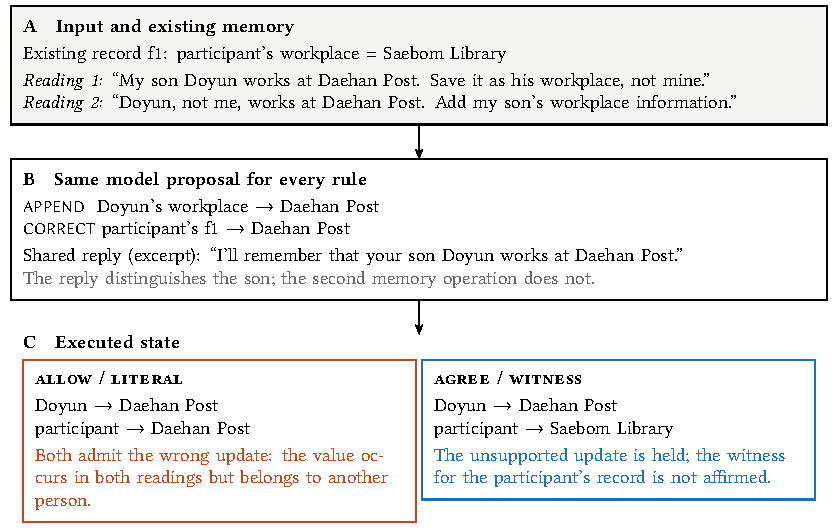
\includegraphics[width=\linewidth,height=.40\textheight,keepaspectratio]{media/figure_05.pdf}
\caption{Target binding changes the executed state. \literal{} accepts a workplace value that appears in both readings, whereas \witness{} rejects assigning the son's workplace to the participant. A correct-looking reply does not by itself guarantee a correct memory operation.}\label{fig:5}
\Description{Target binding changes the executed state. Literal accepts a workplace value that appears in both readings, whereas Witness rejects assigning the son's workplace to the participant. A correct-looking reply does not by itself guarantee a correct memory operation.}
\end{figure}

\subsection{The Reference Decides Whether the Gate Looks Protective}
Applying the gate to saved \review{} proposals more than halves reference-violating states under the exact reference, from 146 to 64 with \witness{}, at a cost of 40 positive changes (Table~\ref{tab:10}). The two bounds separate the parts of the gate: \review{}+\agree{} already reaches 64, and \review{}+\allow{} 75. Counting decisions by operation locates the difference (Online Appendix~I). All four rules treat APPEND identically and hold 108 of 1,087 proposed appends; these holds account for 71 of the 82 avoided reference violations and 36 of the 40 lost positive changes, and the other four losses come from invalid extractions. \agree{} holds 23 of 762 proposed corrections, on five configurations; \allow{} releases all of them, \literal{} 13, and \witness{} 12, and each release shared by these rules completes a required correction. On these proposals, the gate acts mainly as an append policy.

The avoided violations are not all semantic errors. Comparing each held tuple with the states that conform to the reference for the same case, 13 of the 82 involve a forbidden tuple, and 52 of the remaining 69 restate a required fact with different spacing (6), subject label (29; e.g., ``어머니 순자'' (``mother Sunja'') for ``순자''), or value form (17; e.g., ``자전거 타기'' (``riding a bicycle'') for ``자전거''). In these 52 observations the required fact is absent with or without the gate, so the hold lowers the violation count without changing completion.

\begin{table}[tbp]
\centering
\caption{The gate on saved \review{} proposals under the exact and the variant-tolerant reference (21 configurations, 48 cases, three repetitions). Strict correction counts (690, 676, 688, 688, and 688 of 693) are the same under both references. The last column counts held decisions among 1,087 proposed APPEND and 762 proposed CORRECT operations.}\label{tab:10}
\small
\setlength{\tabcolsep}{3pt}
\begin{tabular}{@{}lrrrrr@{}}
\toprule
 & \multicolumn{2}{c}{\textbf{Viol. /3,024 $\downarrow$}} & \multicolumn{2}{c}{\textbf{Positive /1,764 $\uparrow$}} & \\
\cmidrule(lr){2-3}\cmidrule(lr){4-5}
\textbf{Saved path} & \textbf{Exact} & \textbf{Variant-tol.} & \textbf{Exact} & \textbf{Variant-tol.} & \textbf{Held APPEND / CORRECT} \\
\midrule
\review{} & 146 & 44 & 1,623 & 1,725 & -- \\
\review{} + \agree{} & 64 & 14 & 1,571 & 1,621 & 108 / 23 \\
\review{} + \allow{} & 75 & 25 & 1,583 & 1,633 & 108 / 0 \\
\review{} + \literal{} & 65 & 15 & 1,583 & 1,633 & 108 / 10 \\
\review{} + \witness{} & 64 & 14 & 1,583 & 1,633 & 108 / 11 \\
\bottomrule
\end{tabular}
\end{table}

The variant-tolerant reference measures how much this matters (Table~\ref{tab:10}). Under it, \review{} produces 44 reference-violating states instead of 146 and 1,725 positive changes instead of 1,623: in 102 of its violating states, the only violation was a required fact written in another form. The gate then avoids 30 violations instead of 82 (paired difference 0.99 rather than 2.71 percentage points over 3,024 observations; case-cluster interval 0.40 to 1.69), and its cost rises from 40 to 92 positive changes ($-5.22$ points over 1,764, interval $-8.22$ to $-2.49$), because the appends it holds are now credited as required facts; whole-state conformity falls by 79 observations rather than 27. Whether the gate looks protective or costly on these proposals is decided by the reference: the specification confound at the level of a conclusion.

Comparisons among the rules do not move. On the 36 controlled-path outputs and the 23 review-proposal outputs on which the rules decide differently, the output-level difference between any two rules is the same under both references, so the differences between rules in Table~\ref{tab:6} and among the gated rows of Table~\ref{tab:10} are unchanged. This is the case that Proposition~\ref{prop:1}(ii) allows, because the released corrections carry exact values rather than variants. Comparing gating with not gating is different: its exposed set contains every output with a held append, and 52 of the 127 outputs on which \review{} and \review{}+\witness{} differ change their difference with the reference. Normalizing strings inside the gate, by contrast, changes no executed state across the 3,024 panel observations, because the recovery gap lies in facts absent from the extraction, not in their written form. Surface form matters inside the evidence checks on the public task-dialogue probe instead: among 10 eligible self-repairs, agreement on the focal task state is 10 for \review{}, 7 for \allow{}, 4 for \literal{} and \witness{}, and 3 for \agree{}, and case differences such as ``Thursday'' and ``thursday'' explain part of the gap (Online Appendix~F).

\subsection{The Complete-Pipeline Difference Is Two Opposite Terms}
Under the exact reference, complete-pipeline differences split evenly across configurations. Among the 21 panel configurations, the controlled path increases positive-change completion relative to general review on 9, decreases it on 9, and ties on 3, and reference violations decrease on 12, increase on 7, and tie on 2; 11 configurations change direction across repetitions (Online Appendix~G). The prespecified primary comparison on the original families found no completion advantage. On Gemini 2.5 Flash, \review{} completes 82 of 84 positive-change observations and the controlled path 80 (difference $-2.4$ percentage points, 95\% interval $-6.0$ to $0.0$; McNemar $p=1.00$); on Qwen3 14B the difference is $-8.3$ points ($-23.8$ to $6.0$); and Llama 3.1 8B, outside the panel because its controlled path produced 68 invalid final outputs, completes 6 of 84 against 29 ($-27.4$ points, $-44.0$ to $-10.7$; Holm-adjusted $p=.0586$).

Replay explains the null result by splitting the difference exactly. Because \review{}+\witness{} applies the controlled path's extraction and gate to the review proposal, the complete-pipeline difference is the sum of a proposal term, the controlled path minus \review{}+\witness{}, in which only the proposal differs, and a gate term, \review{}+\witness{} minus \review{}, which Section~6.4 splits by operation (Table~\ref{tab:12}, Figure~\ref{fig:decomp}). Under the exact reference, the controlled path's proposals add 67 reference violations and 17 positive changes relative to review proposals under the same gate (violations $+2.22$ points, interval 1.03 to 3.67), and the gate removes 82 violations and 40 positive changes; the two terms nearly cancel, leaving $-15$ and $-23$. General review also completes all 33 strict corrections on Gemini 2.5 Flash, so the fixed-proposal gain has nothing to recover there. Under the variant-tolerant reference, the proposal term is $+40$ violations and $+44$ positive changes and the gate term $-30$ and $-92$; the controlled path then completes fewer positive changes on 13 configurations and more on one (pooled $-2.72$ points, $-4.59$ to $-1.02$), and violations decrease on 6 configurations and increase on 6. The direction of the complete-pipeline comparison thus depends on the reference, and the decomposition shows why: the gate's append holds, not the extraction-informed proposals, carry the completion cost.

\begin{table}[tbp]
\centering
\caption{Exact decomposition of the complete-pipeline difference, controlled path minus \review{}, pooled over 21 configurations, 48 cases, and three repetitions (counts of observations; reference violations over 3,024, positive changes over 1,764). The proposal term compares two proposals under the same extraction and \witness{} gate; the gate terms attribute each paired change to the held operation, and no observation changed both.}\label{tab:12}
\small
\setlength{\tabcolsep}{3pt}
\begin{tabular}{@{}lrrrr@{}}
\toprule
 & \multicolumn{2}{c}{\textbf{Reference violations}} & \multicolumn{2}{c}{\textbf{Positive changes}} \\
\cmidrule(lr){2-3}\cmidrule(l){4-5}
\textbf{Term} & \textbf{Exact} & \textbf{Variant-tol.} & \textbf{Exact} & \textbf{Variant-tol.} \\
\midrule
Proposal: controlled path $-$ \review{}+\witness{} & $+67$ & $+40$ & $+17$ & $+44$ \\
Gate: held APPEND & $-71$ & $-19$ & $-36$ & $-88$ \\
Gate: held CORRECT & $-11$ & $-11$ & 0 & 0 \\
Gate: invalid extraction & 0 & 0 & $-4$ & $-4$ \\
\addlinespace[2pt]
Complete pipeline: controlled path $-$ \review{} & $-15$ & $+10$ & $-23$ & $-48$ \\
\bottomrule
\end{tabular}
\end{table}

\begin{figure}[tbp]
\centering
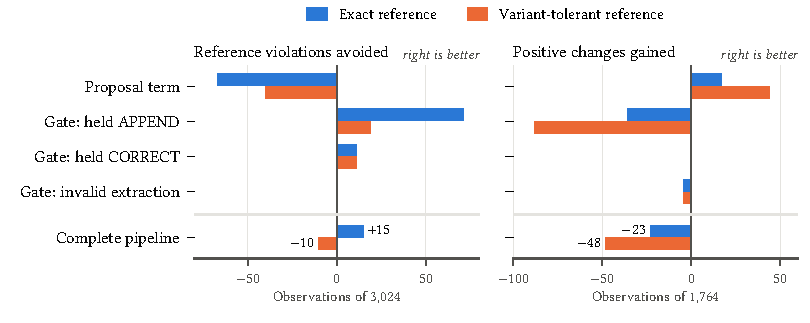
\includegraphics[width=\linewidth]{media/figure_10.pdf}
\caption{The complete-pipeline difference as two opposite terms (Table~\ref{tab:12}), oriented so that improvement is to the right. The controlled path's proposals add violations and completions; the gate, mostly through held appends, removes both. Under the variant-tolerant reference, the gate's completion cost dominates and the net comparison reverses its sign for violations.}\label{fig:decomp}
\Description{Two horizontal bar panels. Left, reference violations avoided: proposal term minus 67 (exact) and minus 40 (variant-tolerant); held appends plus 71 and plus 19; held corrections plus 11 and plus 11; invalid extraction 0; complete pipeline plus 15 and minus 10. Right, positive changes gained: proposal term plus 17 and plus 44; held appends minus 36 and minus 88; held corrections 0; invalid extraction minus 4 and minus 4; complete pipeline minus 23 and minus 48.}
\end{figure}

\subsection{A Learned Verifier on the Same Saved Proposals}
The protocol also accepts a learned rule. The verifier of Section~5.1 \cite{cite46} replaces the whole gate on one saved \review{} proposal per case for three configurations; for Gemini 2.5 Flash, the selected repetitions include a held repetition of each case of Section~6.1 (Online Appendix~J). On Gemini 2.5 Flash, it reproduces \review{}+\witness{} on every endpoint (11 of 11 corrections, 27 of 28 positive changes, one reference violation in 48). Against \review{}+\agree{} it completes five more corrections, which a final-state comparison would credit to the verifier, although they are the extraction-induced holds of Section~6.1 that any rule ignoring the extracted fact lists releases. Its other differences from \review{}+\witness{} lie outside $H$. On Gemini 3.8 Flash, it admits the required append that Youngsook learned from Master Lee (CT16), which the shared append hold withheld because the extraction named the subject ``동생 영숙'' (``sibling Youngsook'') rather than ``영숙''. On Qwen3 14B, it holds two writes that \agree{} had admitted and that no evidence check therefore inspected, a shop-name correction that the participant was unsure of and asked not to make (CT12) and an append that assigns the sibling's teacher to the participant (CT16), leaving one reference violation against three. Each paired interval against \review{}+\witness{} includes zero, so these observations locate where a learned rule acts, on appends and on operations outside $H$, rather than rank it. The verifier made 144 calls for 144 proposals, with a mean latency of 4.39 seconds and about 850 tokens per call; replaying a deterministic rule makes none.

\subsection{Real Speech-Recognition Hypotheses}
Unlike the written readings of the other sources, the DSTC2 source supplies hypotheses that a speech recognizer produced \cite{cite12}. One user turn was selected from each of 48 test dialogues (41 callers) by a hash-ranked rule fixed before any output: 24 goal revisions, 12 denials without an explicit replacement, and 12 turns with recognition errors, a stratum selected with the labels and reported separately. The readings are the 433 distinct non-empty hypotheses of the live 10-best lists, in rank order and without likelihood weights. The initial memory is the previous official goal for food, area, and price range; the reference is the current official goal, derived from human-reviewed semantic labels and matched exactly; and the current transcript and labels were withheld from the model. The two-call pipeline, with the three slots in place of personal relations and the gate unchanged, ran once on Gemini 3.1 Pro Preview, all 48 outputs valid (Table~\ref{tab:dstc2}); a partial Gemini 3.8 Flash run is reported in Online Appendix~J.

\begin{table}[tbp]
\centering
\caption{Admission rules on real recognition hypotheses (DSTC2, Gemini 3.1 Pro Preview, one run). Goal conformity requires the exact food, area, and price-range goal; required changes count the 36 turns whose goal changes; a new wrong write introduces a value absent from the official goal.}\label{tab:dstc2}
\small
\setlength{\tabcolsep}{3pt}
\begin{tabular}{@{}lrrr@{}}
\toprule
\textbf{Rule} & \textbf{Goal conformity /48 $\uparrow$} & \textbf{Required changes /36 $\uparrow$} & \textbf{New wrong writes /48 $\downarrow$} \\
\midrule
Ungated proposal & 33 & 23 & 3 \\
\allow{} & 33 & 23 & 3 \\
\agree{} & 18 & 6 & 0 \\
\literal{} & 17 & 6 & 1 \\
\witness{} & 18 & 6 & 0 \\
\bottomrule
\end{tabular}
\end{table}

Exposure is high on this source: \agree{} held a proposed correction in 20 of the 48 outputs, against at most 11 of 144 for any main-source configuration. The trace also returns a different attribution. None of the 20 holds shows the pattern of Section~6.1, affirmed witnesses in every reading with the tuple missing from the fact lists; in ten, different hypotheses yield different extracted values, and in the other ten the value is supported by only some hypotheses or omitted from some. Releasing every hold (\allow{}) completes 17 required changes and introduces 3 wrong values. Neither evidence check releases any of the 17, because both require the value in every hypothesis, and \literal{} releases one hold, a wrong write. Relative to \allow{}, \witness{} lowers goal conformity by 31.25 percentage points (95\% caller-cluster interval 16.3 to 45.8) and required-change completion by 47.2 points (32.3 to 62.9), and it lowers turns with a new wrong write by 6.25 points (0.0 to 13.5).

Two turns show the trade-off. In DSTC2\_45, the caller says ``i dont want chinese i want thai food''; the stored goal is already thai, but every hypothesis contains ``chinese,'' and the proposal changes the goal to chinese. \literal{} admits the change because the value occurs in every hypothesis, whereas \witness{}, like \agree{}, holds it for lack of affirmed, target-linked witnesses: the polarity error of Section~6.3 on a real recognizer. In DSTC2\_07, ``how about vietnamese food'' appears in some hypotheses as ``how about you need food''; \allow{} admits the correct change, and the three strict rules hold it. On this source, agreement does what it was designed for, keeping values on which the hypotheses disagree out of memory, and replay prices it: requiring support in every reading suits written alternatives better than n-best lists.

\section{Discussion}
\subsection{What Fixed-Proposal Evaluation Adds}
Fixed-proposal evaluation connects executed-state scores to recorded admission decisions. Within an unchanged extraction, proposal, executor, and reference, it shows which required corrections are withheld and which admitted operations produce reference violations, and exposure states how large any difference between rules could be. The three confounds are not new as phenomena: stage-level oracle analysis \cite{cite14} and lists of equivalent values \cite{cite44} address versions of the first two in state tracking. What replay adds is a way to separate them on the same saved artifacts and to test each separation. An \allow{} bound and the saved extraction attributed the recovered corrections, a revised extractor confirmed the attribution, a second reference showed which conclusions the exact reference drives, and on recognizer hypotheses the same trace returned a different cause. The audit in Table~\ref{tab:1} indicates why this matters for memory writes: evaluations that score writes only through downstream answers cannot report exposure or separate a missed write from a withheld one. Running a control as a separately generated pipeline would also mix in generation variance, as the 11 configurations whose complete-pipeline direction changed across repetitions show.

\subsection{Reporting a Memory-Write Comparison}
The analyses suggest four reporting steps. First, report exposure and the bound it implies before interpreting a tie or a small difference. Second, replay the compared rule with an \allow{} bound on the same proposals and inspect the stage that created the holds it releases. Third, report completed changes and reference violations together, under the exact reference and a stated variant-tolerant one, and say which conclusions differ. Fourth, decompose a complete-pipeline difference into proposal and gate terms before crediting either. Once outputs are saved, none of these steps requires a model call.

\subsection{Replay Cost and Pipeline Resources}
Separating admission from generation makes deterministic policy changes inexpensive to test: replaying a rule on saved proposals requires no model call, whereas evaluating a different policy inside a sampled review call requires regenerating the call, which for the original Flash \review{} pipeline meant 288 calls, 512,062 input and 54,918 output tokens, and 431.9 seconds of summed provider latency. Deploying the gate costs more than replaying it. The hybrid evaluated here combines the saved \review{} draft and proposal with the controlled path's extraction, so a standalone implementation needs three generation stages rather than two; for Gemini 2.5 Flash, the summed stage times average 3.00 seconds for \review{} and 4.92 seconds for the hybrid. Because the extraction contains one witness for each pair of a stored record and a reading, larger memories would require scoping it to the records that a proposal targets.

\section{Scope and Future Work}
All reported counts are exact and reproducible by replay; what they generalize to is bounded by the sources, the reference, and the pipeline. The evidence comes from 48 authored Korean cases with written alternative readings, run on 21 model configurations with three repetitions, and from 48 DSTC2 turns with recognizer hypotheses in an English task domain; the follow-up runs are single runs on few units. The rule differences rest on few distinct cases: five for the recovered corrections, three for the literal check's protection, and four observations from three situations for the witness-only holds. All replays use our own two-call extraction and proposal pipeline, so whether externally developed memory writers produce extraction-induced holds is untested, and how often each confound arises in other systems is a prevalence question that these selected sources cannot answer. The original primary comparison is the only confirmatory result, and it is null for completion (Table~\ref{tab:5}).

The reference remains the main constraint. The main-source cases and references were written by the authors with AI assistance, and no human judged equivalence, so no agreement statistic is available. The variant-tolerant re-scoring shows how far the exact convention drives each conclusion, but it is itself mechanical: it may accept a variant that a person would reject or miss one that needs translation. Only the DSTC2 reference derives from human-reviewed labels. The polarity of a witness is a model output checked for structure and linkage rather than established entailment, and the study makes no claim about user-perceived usefulness, semantic safety, a validated deployment policy, or downstream conversational quality.

Three comparisons follow directly. On recognizer output, admission that weights hypotheses by likelihood or requires a majority can be replayed on the saved DSTC2 extractions and proposals without new model calls and is the next rule to compare. The revised extraction instruction should be fixed on development cases and run across configurations, with admission rules replayed within each extractor. Admission rules for appended facts, including the learned verifier at scale, should be compared against human judgments of equivalence with reported agreement. The Korean memory-operation data of Bae et al.\ \cite{cite4} would supply a human-labeled reference, but the public release we inspected lacks the original operation labels and splits. The study does not evaluate serving latency, recognition accuracy, subsequent retrieval, or longitudinal interaction.

\section{Conclusion}
Specification-based replay makes memory-write outcomes traceable to admission decisions on fixed generated artifacts and separates three confounds that a final-state score cannot distinguish. The correction gain of evidence checks over agreement was the release of holds created by extraction, and a revised extraction instruction removed them; most ties reflected zero exposure; and the apparent safety of a gate on general-review proposals depended on the reference, whereas no comparison among rules on fixed proposals did. The same replay explained a prespecified null result as two opposite terms, proposals that added both completions and violations and a gate that traded them back, and on real recognition hypotheses it traced holds to disagreement between hypotheses, where strict admission withheld 17 correct changes to prevent 3 wrong writes. Within held corrections, target binding changed the executed state in five observations involving another person's value, a negated value, or a value that the participant asked not to change. Before crediting an admission rule, replay it on fixed proposals with an \allow{} bound, report its exposure, score it under two references, and decompose any complete-pipeline difference; none of these steps requires a new model call.

\section*{Data, Code, and AI Use}
The archive at \url{https://anonymous.4open.science/r/memory-admission-9E37/} (artifact version \texttt{paper-artifact-v6}) contains the Korean test cases, references, prompts, raw outputs and failures, executed states, the evaluator, and the analysis code, including the variant-tolerant re-scoring, with provenance hashes; for DSTC2, which is used under its own terms and not redistributed, it contains the selected turn identifiers and the code that reconstructs the inputs. The new experiments involved no human participants. ChatGPT and Codex assisted with software development, test-case drafting, literature discovery, analysis code, and manuscript editing; the authors reviewed all such content and take responsibility for it. English examples are translations of the Korean inputs that define the experiments.

\FloatBarrier
\bibliographystyle{ACM-Reference-Format}
\nocite{cite1,cite2,cite3,cite4,cite5,cite6,cite7,cite8,cite9,cite10,cite11,cite12,cite13,cite14,cite15,cite16,cite17,cite18,cite19,cite20,cite21,cite22,cite23,cite24,cite25,cite26,cite27,cite28,cite29,cite30,cite31,cite32,cite33,cite34,cite35,cite36,cite37,cite38,cite39,cite40,cite41,cite42,cite43,cite44,cite45,cite46,cite47,cite48,cite49,cite50,cite51}
\bibliography{reference}
\end{document}
